% Created by tikzDevice version 0.10.1 on 2016-08-31 13:41:48
% !TEX encoding = UTF-8 Unicode
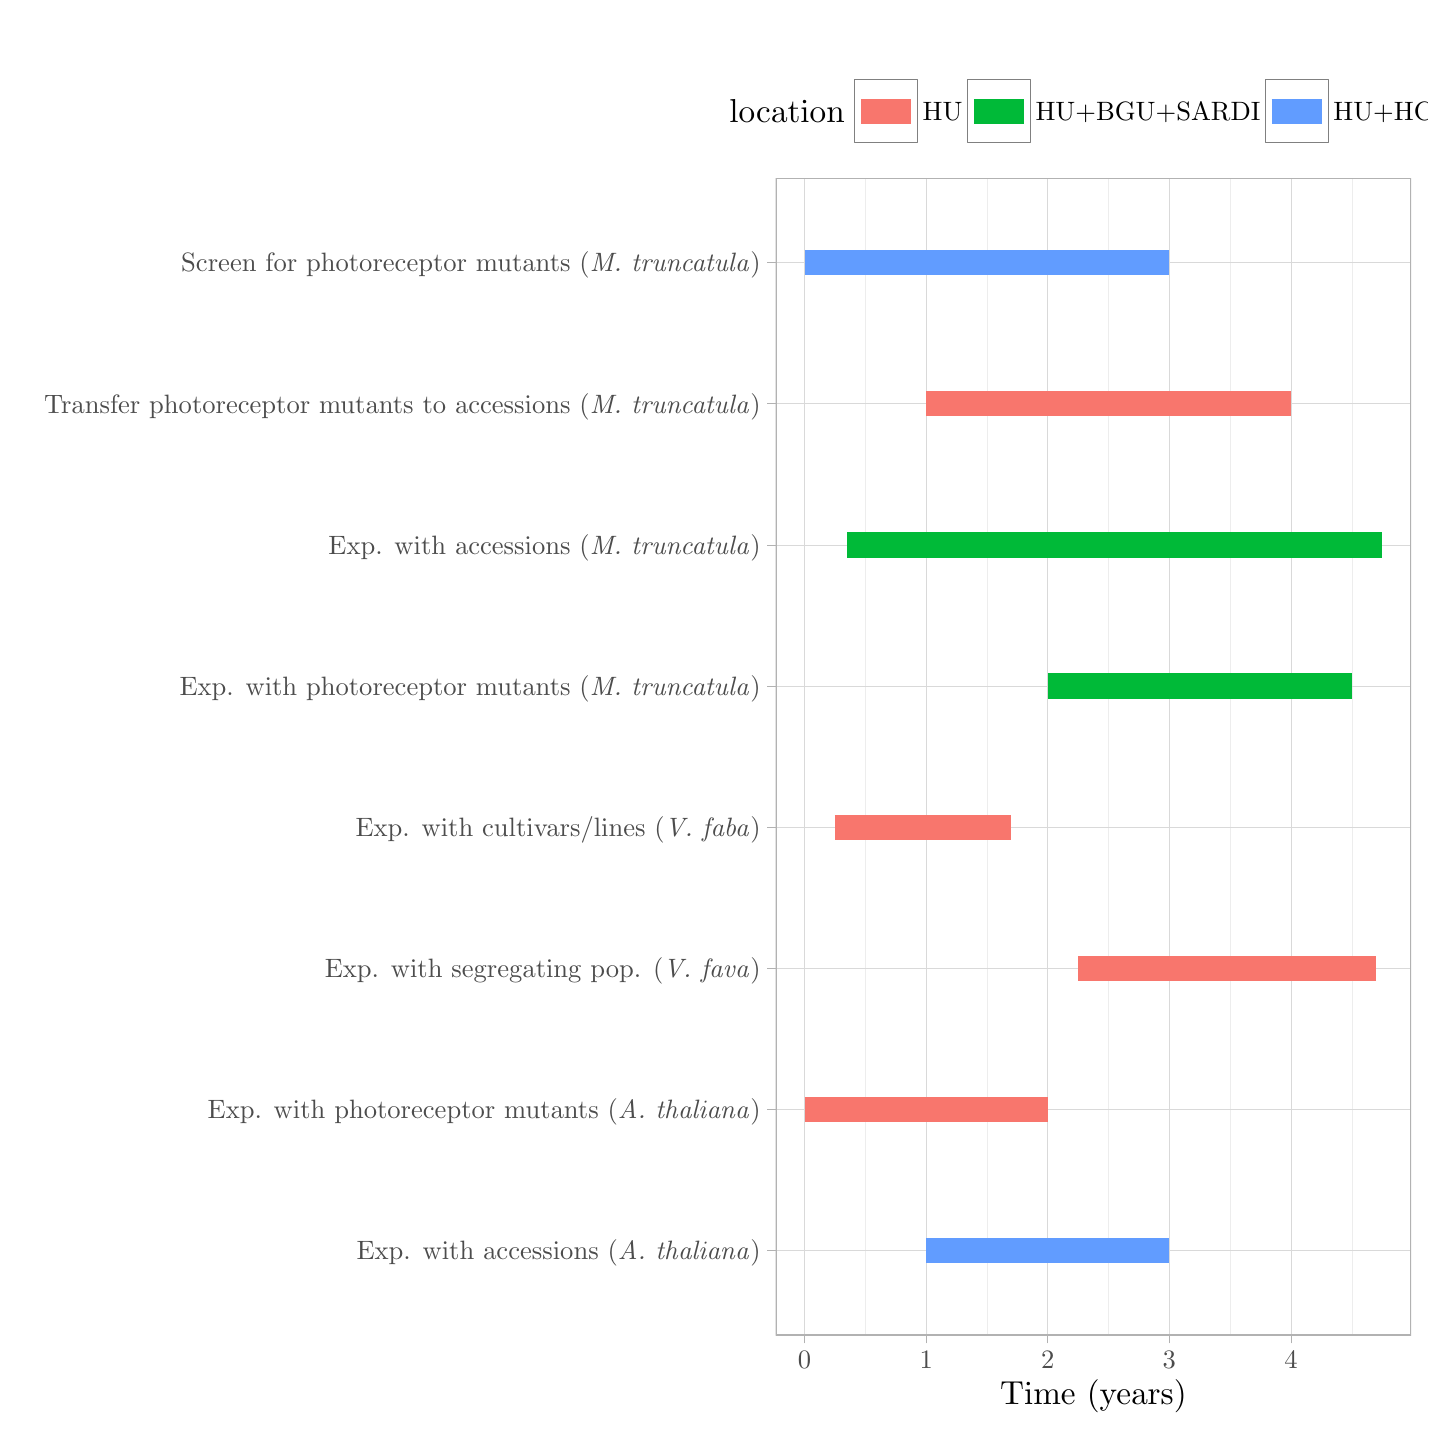
\begin{tikzpicture}[x=1pt,y=1pt]
\definecolor{fillColor}{RGB}{255,255,255}
\path[use as bounding box,fill=fillColor,fill opacity=0.00] (0,0) rectangle (505.89,505.89);
\begin{scope}
\path[clip] (  0.00,  0.00) rectangle (505.89,505.89);
\definecolor{drawColor}{RGB}{255,255,255}
\definecolor{fillColor}{RGB}{255,255,255}

\path[draw=drawColor,line width= 0.6pt,line join=round,line cap=round,fill=fillColor] (  0.00,  0.00) rectangle (505.89,505.89);
\end{scope}
\begin{scope}
\path[clip] (270.29, 33.48) rectangle (499.89,451.52);
\definecolor{fillColor}{RGB}{255,255,255}

\path[fill=fillColor] (270.29, 33.48) rectangle (499.89,451.52);
\definecolor{drawColor}{gray}{0.93}

\path[draw=drawColor,line width= 0.1pt,line join=round] (302.70, 33.48) --
	(302.70,451.52);

\path[draw=drawColor,line width= 0.1pt,line join=round] (346.64, 33.48) --
	(346.64,451.52);

\path[draw=drawColor,line width= 0.1pt,line join=round] (390.58, 33.48) --
	(390.58,451.52);

\path[draw=drawColor,line width= 0.1pt,line join=round] (434.52, 33.48) --
	(434.52,451.52);

\path[draw=drawColor,line width= 0.1pt,line join=round] (478.47, 33.48) --
	(478.47,451.52);
\definecolor{drawColor}{gray}{0.85}

\path[draw=drawColor,line width= 0.3pt,line join=round] (270.29, 64.06) --
	(499.89, 64.06);

\path[draw=drawColor,line width= 0.3pt,line join=round] (270.29,115.05) --
	(499.89,115.05);

\path[draw=drawColor,line width= 0.3pt,line join=round] (270.29,166.03) --
	(499.89,166.03);

\path[draw=drawColor,line width= 0.3pt,line join=round] (270.29,217.01) --
	(499.89,217.01);

\path[draw=drawColor,line width= 0.3pt,line join=round] (270.29,267.99) --
	(499.89,267.99);

\path[draw=drawColor,line width= 0.3pt,line join=round] (270.29,318.97) --
	(499.89,318.97);

\path[draw=drawColor,line width= 0.3pt,line join=round] (270.29,369.95) --
	(499.89,369.95);

\path[draw=drawColor,line width= 0.3pt,line join=round] (270.29,420.93) --
	(499.89,420.93);

\path[draw=drawColor,line width= 0.3pt,line join=round] (280.72, 33.48) --
	(280.72,451.52);

\path[draw=drawColor,line width= 0.3pt,line join=round] (324.67, 33.48) --
	(324.67,451.52);

\path[draw=drawColor,line width= 0.3pt,line join=round] (368.61, 33.48) --
	(368.61,451.52);

\path[draw=drawColor,line width= 0.3pt,line join=round] (412.55, 33.48) --
	(412.55,451.52);

\path[draw=drawColor,line width= 0.3pt,line join=round] (456.50, 33.48) --
	(456.50,451.52);
\definecolor{drawColor}{RGB}{248,118,109}

\path[draw=drawColor,line width= 9.1pt,line join=round] (280.72,115.05) --
	(368.61,115.05);

\path[draw=drawColor,line width= 9.1pt,line join=round] (379.60,166.03) --
	(487.26,166.03);

\path[draw=drawColor,line width= 9.1pt,line join=round] (291.71,217.01) --
	(355.43,217.01);

\path[draw=drawColor,line width= 9.1pt,line join=round] (324.67,369.95) --
	(456.50,369.95);
\definecolor{drawColor}{RGB}{0,186,56}

\path[draw=drawColor,line width= 9.1pt,line join=round] (368.61,267.99) --
	(478.47,267.99);

\path[draw=drawColor,line width= 9.1pt,line join=round] (296.10,318.97) --
	(489.45,318.97);
\definecolor{drawColor}{RGB}{97,156,255}

\path[draw=drawColor,line width= 9.1pt,line join=round] (324.67, 64.06) --
	(412.55, 64.06);

\path[draw=drawColor,line width= 9.1pt,line join=round] (280.72,420.93) --
	(412.55,420.93);
\definecolor{drawColor}{gray}{0.70}

\path[draw=drawColor,line width= 0.6pt,line join=round,line cap=round] (270.29, 33.48) rectangle (499.89,451.52);
\end{scope}
\begin{scope}
\path[clip] (  0.00,  0.00) rectangle (505.89,505.89);
\definecolor{drawColor}{gray}{0.30}

\node[text=drawColor,anchor=base east,inner sep=0pt, outer sep=0pt, scale=  0.96] at (264.89, 60.76) {Exp. with accessions (\emph{A. thaliana})};

\node[text=drawColor,anchor=base east,inner sep=0pt, outer sep=0pt, scale=  0.96] at (264.89,111.74) {Exp. with photoreceptor mutants (\emph{A. thaliana})};

\node[text=drawColor,anchor=base east,inner sep=0pt, outer sep=0pt, scale=  0.96] at (264.89,162.72) {Exp. with segregating pop. (\emph{V. fava})};

\node[text=drawColor,anchor=base east,inner sep=0pt, outer sep=0pt, scale=  0.96] at (264.89,213.70) {Exp. with cultivars/lines (\emph{V. faba})};

\node[text=drawColor,anchor=base east,inner sep=0pt, outer sep=0pt, scale=  0.96] at (264.89,264.68) {Exp. with photoreceptor mutants (\emph{M. truncatula})};

\node[text=drawColor,anchor=base east,inner sep=0pt, outer sep=0pt, scale=  0.96] at (264.89,315.66) {Exp. with accessions (\emph{M. truncatula})};

\node[text=drawColor,anchor=base east,inner sep=0pt, outer sep=0pt, scale=  0.96] at (264.89,366.64) {Transfer photoreceptor mutants to accessions (\emph{M. truncatula})};

\node[text=drawColor,anchor=base east,inner sep=0pt, outer sep=0pt, scale=  0.96] at (264.89,417.63) {Screen for photoreceptor mutants (\emph{M. truncatula})};
\end{scope}
\begin{scope}
\path[clip] (  0.00,  0.00) rectangle (505.89,505.89);
\definecolor{drawColor}{gray}{0.70}

\path[draw=drawColor,line width= 0.3pt,line join=round] (267.29, 64.06) --
	(270.29, 64.06);

\path[draw=drawColor,line width= 0.3pt,line join=round] (267.29,115.05) --
	(270.29,115.05);

\path[draw=drawColor,line width= 0.3pt,line join=round] (267.29,166.03) --
	(270.29,166.03);

\path[draw=drawColor,line width= 0.3pt,line join=round] (267.29,217.01) --
	(270.29,217.01);

\path[draw=drawColor,line width= 0.3pt,line join=round] (267.29,267.99) --
	(270.29,267.99);

\path[draw=drawColor,line width= 0.3pt,line join=round] (267.29,318.97) --
	(270.29,318.97);

\path[draw=drawColor,line width= 0.3pt,line join=round] (267.29,369.95) --
	(270.29,369.95);

\path[draw=drawColor,line width= 0.3pt,line join=round] (267.29,420.93) --
	(270.29,420.93);
\end{scope}
\begin{scope}
\path[clip] (  0.00,  0.00) rectangle (505.89,505.89);
\definecolor{drawColor}{gray}{0.70}

\path[draw=drawColor,line width= 0.3pt,line join=round] (280.72, 30.48) --
	(280.72, 33.48);

\path[draw=drawColor,line width= 0.3pt,line join=round] (324.67, 30.48) --
	(324.67, 33.48);

\path[draw=drawColor,line width= 0.3pt,line join=round] (368.61, 30.48) --
	(368.61, 33.48);

\path[draw=drawColor,line width= 0.3pt,line join=round] (412.55, 30.48) --
	(412.55, 33.48);

\path[draw=drawColor,line width= 0.3pt,line join=round] (456.50, 30.48) --
	(456.50, 33.48);
\end{scope}
\begin{scope}
\path[clip] (  0.00,  0.00) rectangle (505.89,505.89);
\definecolor{drawColor}{gray}{0.30}

\node[text=drawColor,anchor=base,inner sep=0pt, outer sep=0pt, scale=  0.96] at (280.72, 21.46) {0};

\node[text=drawColor,anchor=base,inner sep=0pt, outer sep=0pt, scale=  0.96] at (324.67, 21.46) {1};

\node[text=drawColor,anchor=base,inner sep=0pt, outer sep=0pt, scale=  0.96] at (368.61, 21.46) {2};

\node[text=drawColor,anchor=base,inner sep=0pt, outer sep=0pt, scale=  0.96] at (412.55, 21.46) {3};

\node[text=drawColor,anchor=base,inner sep=0pt, outer sep=0pt, scale=  0.96] at (456.50, 21.46) {4};
\end{scope}
\begin{scope}
\path[clip] (  0.00,  0.00) rectangle (505.89,505.89);
\definecolor{drawColor}{RGB}{0,0,0}

\node[text=drawColor,anchor=base,inner sep=0pt, outer sep=0pt, scale=  1.20] at (385.09,  8.40) {Time (years)};
\end{scope}
\begin{scope}
\path[clip] (  0.00,  0.00) rectangle (505.89,505.89);
\definecolor{fillColor}{RGB}{255,255,255}

\path[fill=fillColor] (249.31,460.06) rectangle (520.87,491.35);
\end{scope}
\begin{scope}
\path[clip] (  0.00,  0.00) rectangle (505.89,505.89);
\definecolor{drawColor}{RGB}{0,0,0}

\node[text=drawColor,anchor=base west,inner sep=0pt, outer sep=0pt, scale=  1.20] at (253.58,471.57) {location};
\end{scope}
\begin{scope}
\path[clip] (  0.00,  0.00) rectangle (505.89,505.89);
\definecolor{drawColor}{gray}{0.50}
\definecolor{fillColor}{RGB}{255,255,255}

\path[draw=drawColor,line width= 0.3pt,line join=round,line cap=round,fill=fillColor] (298.85,464.32) rectangle (321.61,487.09);
\end{scope}
\begin{scope}
\path[clip] (  0.00,  0.00) rectangle (505.89,505.89);
\definecolor{drawColor}{RGB}{248,118,109}

\path[draw=drawColor,line width= 9.1pt,line join=round] (301.12,475.71) -- (319.33,475.71);
\end{scope}
\begin{scope}
\path[clip] (  0.00,  0.00) rectangle (505.89,505.89);
\definecolor{drawColor}{gray}{0.50}
\definecolor{fillColor}{RGB}{255,255,255}

\path[draw=drawColor,line width= 0.3pt,line join=round,line cap=round,fill=fillColor] (339.62,464.32) rectangle (362.38,487.09);
\end{scope}
\begin{scope}
\path[clip] (  0.00,  0.00) rectangle (505.89,505.89);
\definecolor{drawColor}{RGB}{0,186,56}

\path[draw=drawColor,line width= 9.1pt,line join=round] (341.90,475.71) -- (360.11,475.71);
\end{scope}
\begin{scope}
\path[clip] (  0.00,  0.00) rectangle (505.89,505.89);
\definecolor{drawColor}{gray}{0.50}
\definecolor{fillColor}{RGB}{255,255,255}

\path[draw=drawColor,line width= 0.3pt,line join=round,line cap=round,fill=fillColor] (447.24,464.32) rectangle (470.00,487.09);
\end{scope}
\begin{scope}
\path[clip] (  0.00,  0.00) rectangle (505.89,505.89);
\definecolor{drawColor}{RGB}{97,156,255}

\path[draw=drawColor,line width= 9.1pt,line join=round] (449.52,475.71) -- (467.73,475.71);
\end{scope}
\begin{scope}
\path[clip] (  0.00,  0.00) rectangle (505.89,505.89);
\definecolor{drawColor}{RGB}{0,0,0}

\node[text=drawColor,anchor=base west,inner sep=0pt, outer sep=0pt, scale=  0.96] at (323.42,472.40) {HU};
\end{scope}
\begin{scope}
\path[clip] (  0.00,  0.00) rectangle (505.89,505.89);
\definecolor{drawColor}{RGB}{0,0,0}

\node[text=drawColor,anchor=base west,inner sep=0pt, outer sep=0pt, scale=  0.96] at (364.19,472.40) {HU+BGU+SARDI};
\end{scope}
\begin{scope}
\path[clip] (  0.00,  0.00) rectangle (505.89,505.89);
\definecolor{drawColor}{RGB}{0,0,0}

\node[text=drawColor,anchor=base west,inner sep=0pt, outer sep=0pt, scale=  0.96] at (471.81,472.40) {HU+HCM};
\end{scope}
\end{tikzpicture}
